\documentclass[10pt,a4paper]{report}
\usepackage[utf8]{inputenc}
\usepackage{amsmath}
\usepackage{amsfonts}
\usepackage{amssymb}
\usepackage{graphicx}
\usepackage{tabto}
\usepackage{tocloft}
\usepackage[margin=1in]{geometry}
\author{Finn Matras, Jakob Løver}
\title{{\LARGE TFY4115}\\{\large Lab 1, Friksjon på skråplan}}
\begin{document}
\renewcommand{\contentsname}{Innhold}
\renewcommand{\cftchapleader}{\cftdotfill{\cftdotsep}}
\renewcommand{\cftpartleader}{\cftdotfill{\cftdotsep}}

\maketitle
\tableofcontents
%\chapter*{Innhold}
%\begin{itemize}
%\item Sammendrag \tab{1}			
%\item Innledning \tab{2}
%\item Teori      \tab{3}
%\item Eksperimentelt \tab{4}
%\item Resultater og diskusjon \tab{5}
%\item Konklusjon \tab{6}
%\end{itemize}

\chapter*{Sammendrag}
\addcontentsline{toc}{chapter}{Sammendrag}
I dette forsøket ble friksjonskoeffisienter til to ulike stoffer funnet, for at man skal kunne regne seg fram til en den horisontale vinkelen til skråplanet som gjør at et system bestående av to masser sklir med konstant hanstighet ned skråplanet.\\
\\For å finne friksjonskoeffisienten bruke vi videoanalyse-programvaren Tracker og et høyhastighetskamera for å analysere bevegelsen til klossene. I Tracker kunne vi lese av akselerasjonen til klossen, og ved hjelp av Newtons II lov kunne vi regne oss frem til friksjonskoeffisienten til underlagene. Målingene ble gjenntatt flere ganger for å verifisere og ta høyde for usikkerhet.\\
\\Vi fant ut at friksjonskoeffisienten mellom nylon (Figur: 1) og skråplanet i tre var: 0.232, og at friksjonskoeffisienten mellom plast og tre (Figur: 2) var: 0.270.


\chapter*{Innledning}
\addcontentsline{toc}{chapter}{Innledning}
\begin{figure}[p]
    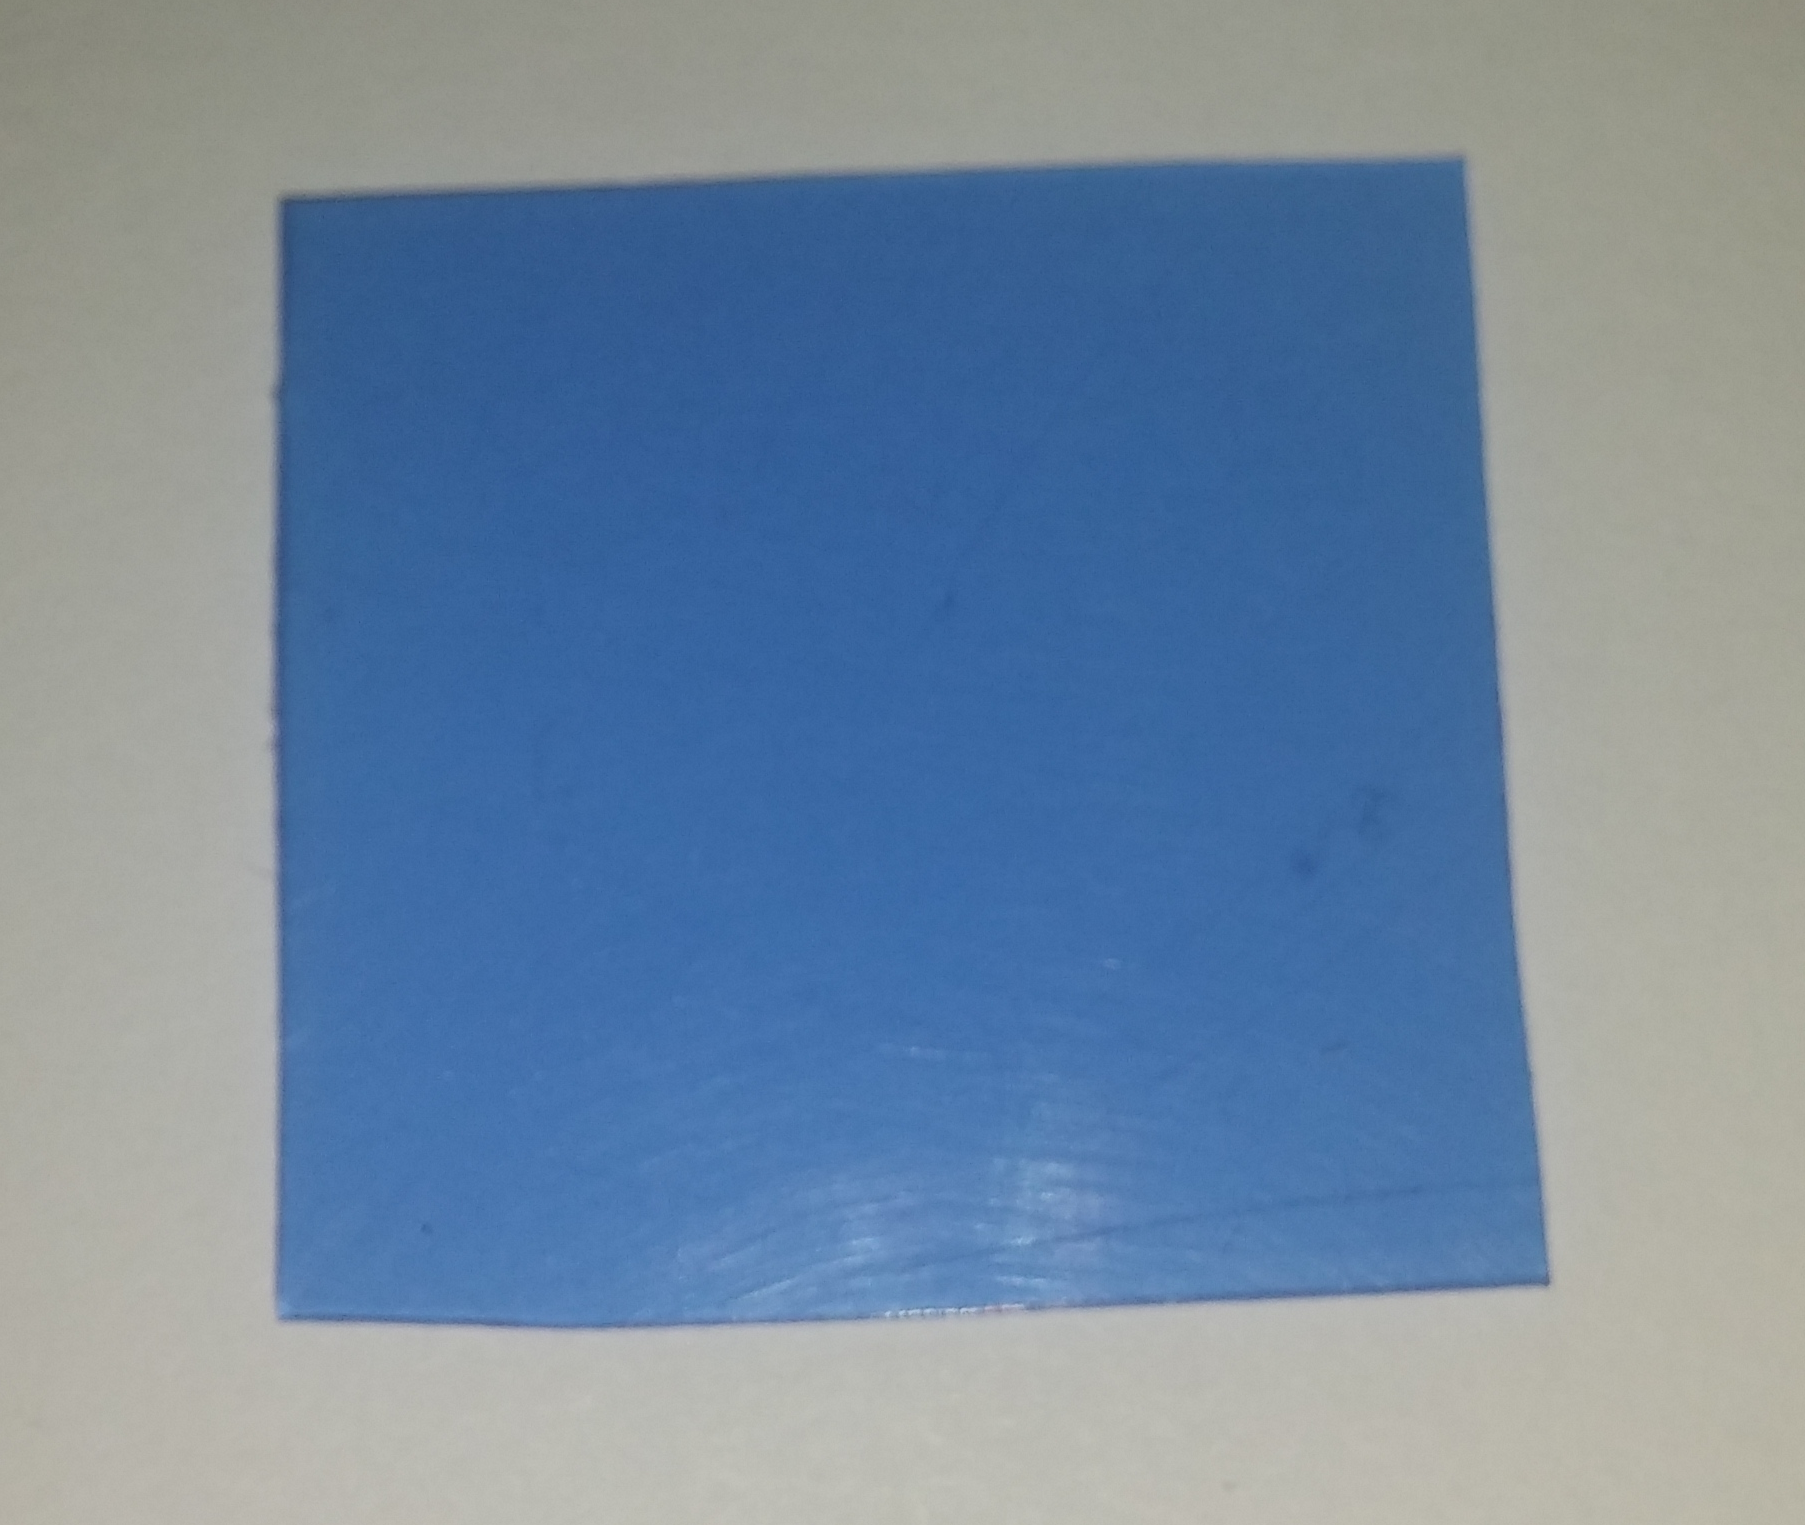
\includegraphics[scale=0.05]{BlaaPlast}
    \caption{Plast, friksjonskoeffisient: 234324324}
    \label{fig:1}
\end{figure}
\begin{figure}[p]
    \includegraphics[scale=0.05]{GultStoff}
    \caption{Nylon, friksjonskoeffisient: 234324324}
    \label{fig:2}
\end{figure}
\section*{Teori}
Basert på Newtons II lov som i likning (2): 
\begin{equation}
\sum{F} = m*a,
\end{equation} der $F$ er kraften, $m$ er massen, og $a$ er akselerasjonen, så kan vi regne ut kreftene som er tilstede på en masse. Hvis $a$ er 0, så får man likning (2) for klossene i figur 3. 
\begin{equation}
F = \mu *F_n
\end{equation}
Likning (3) brukes til å regne ut friksjonskoeffisienten, $\mu$. Ved å regne på likningene over, så får vi likning (1) og (4)
\begin{equation}
\mu = tan(\theta)-a/(cos(\theta)*g)
\end{equation}
Vi kan så bruke denne liknignen til å regne ut friksjonskoeffisienten for de forskjellige akselerasjonsmålingene. Se figur 324532432423. 
\begin{equation}
\theta = arctan(\frac{\mu_1*m_1+\mu_2*m_2}{m_1+m_2})
\end{equation}
Ved hjelp av likning (1) kan man så regne seg fram til vinkelen, $\theta$, som gjør at klossene med masser $m_1$ og $m_2$ sklir med konstant fart ned langs skråplanet for et massesystem på et gitt underlag med friksjonskoeffisient, $\mu$.\\
\\I dette forsøket var formålet å bli kjent med hvordan man utfører forsøk i fysikken, og å bli kjent med hvordan man skriver lab-journal og rapport. Vi har lært mye om usikkerhet og hvordan feil i det tekniske utstyret kan føre til følgefeil. Videre har vi også lært oss hvordan vi bør føre journal for at vi eller andre i etterkant selv skal kunne gjennomføre forsøket på nytt.

\chapter*{Utstyr og metoder}
\addcontentsline{toc}{chapter}{Utstyr og metoder}
\section*{Forberedelse}
\addcontentsline{toc}{subsection}{Forberedelse}
Oppsettet til laben er illustrert i Figure \ref{oppsett}. Et skråplan i treverk er festet til labstativet med en klype. Et vater ble brukt for at vinkelen til skråplanet ble målt relativt til tyngekraten. Foran oppsettet ligger det en meterstokk, noe som gjør det enkelt å kalibrere oppsettet i Tracker. Høyhastighetskameraet er montert normalt på oppsettet, slik at vinkling på kameraet ikke påvirker størrelsene vi måler. Til forsøket ble det brukt to forskjellige klosser: en av messing, og en av aluminium. De forskjellige underlagene ble festet på klossene ved hjelp av lærertyggis.\\
\\For å forberede oss til laben kalkulerte vi først ut likningene vi kom til å bruke under laben, som er beskrevet under seksjonen "Teori." Vi lagde deretter et spreadsheet hvor vi plugget inn alle likningene og størrelsene våre. Dette gjorde at vi kunne enkelt gjøre mange kalkulasjoner av gangen uten å måtte bruke kalkulator for hver gang. Vi stilte inn innstillingene på høyhastighetskameraet tilpasset lysforholdene på laben. Dette resulterte i at vi brukte 100fps fordi det gav best resultater i Tracker.\\
\\En rekke eksperimenter ble fullført for å verifisere at utstyret vårt fungerte. Ved hjelp av en vekt målte vi de to massenes vekt tre ganger. Vi brukte gjennomsnittet av de tre målingene for å være sikre på at vi hadde fått representative tall. Deretter slapp vi en av vektene foran en hvit vegg mens vi filmet med kameraet. Dette importerte vi i Tracker, og ved hjelp av regresjonsfunksjonen i programmet kunne vi verifisere integriteten da vi målte 9.81 m/s$^2$ som akselerasjon.

\section*{Forsøk}
\addcontentsline{toc}{subsection}{Forsøk}
Forsøket ble gjennomført ved å først stille inn skråplanet til riktig vinkel. Med en linjal målte vi lengden og høyden av skråplanet, og brukte den inverse tangensen for å kalkulere vinkelen til skråplanet. Når kameraet rullet, slapp vi messingklossen 4 ganger nedover skråplanet. Dette importerte vi i Tracker for å beregne akselerasjon. Ved hjelp av regnearket vårt og formlene definert ovenfor, regnet vi oss fram til friksjonskoeffesienten for messingklossen. Dette gjentok vi med aluminiumsklossen, og deretter med både nylonbiten og plastbiten som underlag. \\
\\Friksjonskoeffesientene for underlagene vi valgte brukte vi til å beregne oss frem til den optimale vinkelen hvor begge klossene ville skli med konstant hastighet, som beskrevet i "Teori" seksjonen. Klossene ble bundet sammen med en tråd, og sluppet ned skråplanet. Dette forsøket ble også tatt opp ved hjelp av Tracker hvor vi målte en neglisjerbar akselerasjon, noe som bekreftet beregningene våre om optimal vinkel.\\
\\Til slutt ble vi bedt om å kalkulere optimal vinkel da det ble lagt til ulik masse på hver av klossene. Da vi allerede hadde kalkulert friksjonskoeffesientene til underlagene i de forrige eksperimentene, kunne vi enkelt kalkulere vinkelen med de samme formlene. Denne gangen målte vi også en neglisjerbar akselerasjon.

\begin{figure}
\centerline{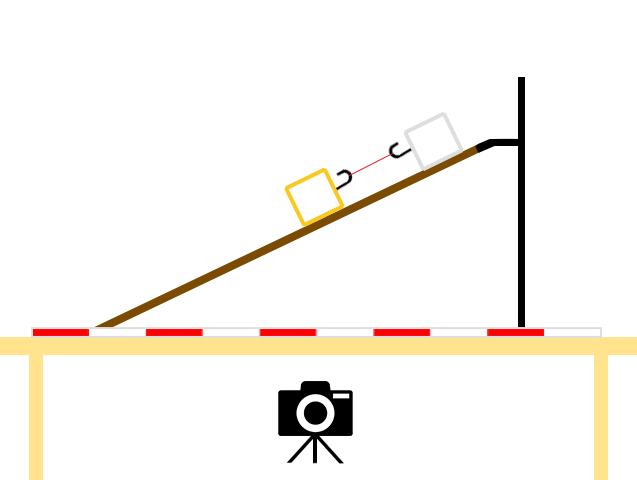
\includegraphics[scale=0.5]{oppsett}}
\caption{Illustrasjon av oppsettet}
\label{oppsett}
\end{figure}

\chapter*{Resultater og diskusjon}
\addcontentsline{toc}{chapter}{Resultater og diskusjon}
\section*{Resultater}
\addcontentsline{toc}{section}{Resultater}
Nedenfor er resultatene vi fikk ved å bruke Tracker til å finne akselerasjonen til klossene, og usikkerheten til disse målingene.
\begin{center}
  \begin{tabular}{| c | c | c | c | c | c |}
    \hline
    Måling & Klosstype & Materiale & Akselerasjon [m/s$^2$] & Vinkel [$\deg$] & Friksjonskoeffisient | \\ \hline
    1 & Messing & Nylon & 0,248 & 17,8 & 0,268 \\ \hline
    2 & Messing & Nylon & 0,412 & 16,9 & 0,216 \\ \hline
    3 & Messing & Nylon & 0,37 & 16,8 & 0,223 \\ \hline
    4 & Messing & Nylon & 0,366 & 16,7 & 0,222 \\ \hline
    Snitt & Messing & Nylon & 0,349 & 17,1 & 0,232 \\ \hline
    Avvik & Messing & Nylon & 0,082 & 0,55 & 0,0260 \\
    \hline
  \end{tabular}
\end{center}


\begin{center}
  \begin{tabular}{| c | c | c | c | c | c |}
    \hline
    Måling & Klosstype & Materiale & Akselerasjon [m/s$^2$] & Vinkel [$\deg$] & Friksjonskoeffisient | \\ \hline
    5 & Aluminium & Nylon & 0,339 & 17,2 & 0,237 \\ \hline
    6 & Aluminium & Nylon & 0,299 & 16,8 & 0,238 \\ \hline
    7 & Aluminium & Nylon & 0,294 & 17,8 & 0,258 \\ \hline
    8 & Aluminium & Nylon & 0,306 & 17,5 & 0,250 \\ \hline
    Snitt & Aluminium & Nylon & 0,310 & 17,3 & 0,246 \\ \hline
    Avvik & Aluminium & Nylon & 0,023 & 0,50 & 0,011 \\
    \hline
  \end{tabular}
\end{center}


\begin{center}
  \begin{tabular}{| c | c | c | c | c | c |}
    \hline
    Måling & Klosstype & Materiale & Akselerasjon [m/s$^2$] & Vinkel [$\deg$] & Friksjonskoeffisient | \\ \hline
    9 & Messing & Plast & 0,337 & 18,2 & 0,256 \\ \hline
    10 & Messing & Plast & 0,196 & 18,7 & 0,296 \\ \hline
    11 & Messing & Plast & 0,296 & 17,8 & 0,258 \\ \hline
    12 & Messing & Plast & 0,189 & 18,2 & 0,288 \\ \hline
    Snitt & Messing & Plast & 0,255 & 18,2 & 0,27 \\ \hline
    Avvik & Messing & Plast & 0,074 & 0,45 & 0,020 \\
    \hline
  \end{tabular}
\end{center}

For å beregne farten til aluminiumsklossen med plastunderlag, så måtte vi endre vinkelen for at klossen skulle skli.
\begin{center}
  \begin{tabular}{| c | c | c | c | c | c |}
    \hline
    Måling & Klosstype & Materiale & Akselerasjon [m/s$^2$] & Vinkel [$\deg$] & Friksjonskoeffisient | \\ \hline
    13 & Aluminium & Plast & 0,431 & 25 & 0,369 \\ \hline
    14 & Aluminium & Plast & 0,418 & 24,9 & 0,370 \\ \hline
    15 & Aluminium & Plast & 0,572 & 26,1 & 0,360 \\ \hline
    16 & Aluminium & Plast & 0,766 & 25,3 & 0,300 \\ \hline
    Snitt & Aluminium & Plast & 0,547 & 25,3 & 0,350 \\ \hline
    Avvik & Aluminium & Plast & 0,174 & 0,60 & 0,035 \\
    \hline
  \end{tabular}
\end{center}

Ved å sette verdiene for snitt, med usikkerhet inn i linkning (1), og få følgende verdier for vinkelen, $\theta$, for et system bestående av to klosser som i illustrasjon 32234532423432:

\begin{center}
  \begin{tabular}{| c | c | c | c | c |}
    \hline
    Stoff kloss 1 & Stoff kloss 2 & $\theta_snitt$ & $\theta_maks$ & $\theta_min$ | \\ \hline
    Nylon & Nylon & 13,6 & 14,4 & 12,8 \\ \hline
    Plast & Plast & 16,4  & 17,6 & 15,1 \\ \hline
    Nylon & Plast & 17,7 & 19,4 & 15,2 \\ \hline
    Plast & Nylon & 14,7 & 16,2 & 13,2  \\ \hline
  \end{tabular}
\end{center}

Testing av utregnede verdier på et massesystem som vist i Figure \ref{oppsett} ga oss følgende akselerasjoner:

\begin{center}
  \begin{tabular}{| c | c | c | c | c  | c |}
    \hline
    Test nr. & Stoff & Vekt kloss 1 & Vekt kloss 2 & Vinkel $\theta$ & Akselerasjon $[m/s^2]$ | \\ \hline
    1 & Nylon & 0,022 & 0,0687 & 12,8 & 0,12 \\ \hline
    2 & Nylon & 0,0242  & 0,0687 & 12,4 & 0,0216 \\ \hline
    3 & Nylon & 0,0343 & 0,1197 & 12,9 & 0,04 \\ \hline
    4 & Plast & 0,0343 & 0,1197 & 16 & lav  \\ \hline
  \end{tabular}
\end{center}

\section*{Diskusjon og feilkilder}
\addcontentsline{toc}{section}{Diskusjon og feilkilder}
Som vi ser i resultatene ovenfor, så ga alle de teoretisk utregnede verdiene en vinkel som var for stor, noe som førte til at klossene akselererte nedover skråplanet. En feilkilde som ble observert mens vi gjennomførte disse testene som hadde ensten konstant hastighet var at klossene beveget seg litt hakkete nedover skråplanet. Dette er mest sannsynlig forårsaket ved at skråplanet ikke har helt monoton overflate, noe som gjør at klossene og friksjonskoeffisientene endrer seg underveis. Vi klarte heller ikke å slippe klossene ned på akuratt samme sted, da skråplanet var forholdsvis bredt, og overflaten kan også være forskjellig i bredden, noe som kan ha forårsaket feil i målingne. Ut ifra likningen ser man også at vinkelen, $\theta$ har mye å si, og dette merket vi også i starten da vi gjorde noen initielle målinger. Det at vi bruke et vater til å finne nøyaktig horisontal posisjon var svært viktig, men her kan det fortsatt være en del usikkerhet, med tanke på hvordan det ble overført til Tracker. \\
\\På måling 13 til 16 ser vi også at friksjonskoeffisienten er en del større, enn den er på måling 9 til 12. Her har vi både endret massen, og vinkelen. Vel å merke her er at det er forskjell på friksjon avhengig av forskjellen i hastighet mellom de to underlagene. Det vil si at for plast var det en annen friksjonskoeffisient ved høyere hastigheter enn ved lavere hastigheter. Det vil si at det kunne vært lurt å prøve seg fram til den vinkelen der det er konstant hastighet eksperimentelt, og så analysere akselerasjonen ved den funnede vinkelen for å finne friksjonskoeffisienten slik den er i nærheten av den hastigheten som den kommer til å bli utsatt for.\\
\\En annen ting vi merket ved målingene som vi gjorde helt i starten av en kloss i fritt fall, var at selv om klossen falt fritt, så stemte ikke alltid akselerasjonsverdiene som vi fikk ved regresjonen i Tracker. Det vi så var at disse verdiene lå i nærheten av det vi skulle forvente, men at verdiene hadde en usikkerhet på rundt $\pm 20 prosent$. Derfor valgte vi å ta totalt 8 målinger av hver stofftype, men for enda mer presise resultater kunne det blitt gjort en rekke flere målinger.
\chapter*{Konklusjon}
\addcontentsline{toc}{chapter}{Konklusjon}
Hypotesen vår var at vi ville klare å kalkulere optimal vinkel for konstant akselerasjon, noe vi kan konkludere med at vi klarte. Det var en del feilkilder som gjorde at resultatene våre ikke ble slik vi håpet på som beskrevet i seksjonen over. Vi opplevde ofte at vi fikk en for høy vinkel da vi kalkulerte vinkelen, noe vi så var et gjengående moment hos de andre gruppene. Etter å ha sammenliknet friksjonskoeffisientene til underlagene med nettet, kan vi også konkludere at vi klarte dette. Utfordringen hvor vi ble bedt om å finne vinkel til to forskjellige masser med eget valg av friksjonsunderlag klarte vi også å bestå, dog med samme problem hvor vi måtte senke planet med et par graders avvik fra beregningene våre. 
\end{document}